% LaTeX file for a 1 page document
\documentclass[12pt]{report}
\usepackage{amsmath}
\usepackage{amssymb}
\usepackage{amsthm}
%\usepackage{physymb}
\usepackage{graphicx}
%\usepackage{wrapfig}
\bibliographystyle{plain}
\usepackage{tikz}
\usepackage{natbib}
\usetikzlibrary{calc,patterns,decorations.pathmorphing,decorations.markings}

\title{Simulation of an Orrery in Box2D\\ A CS296 Report by Group 07}
\author{Ranveer Aggarwal (120050020) \\ ranveeraggarwal@gmail.com \and Devdeep Ray (120050007) \\ devdeep.ray1994@iitb.ac.in \and Sasibhushan Rallabandi (120050056) \\ sasiralla@iitb.ac.in}
\date{}

\begin{document}
\maketitle

\chapter*{Introduction}
An orrery is a mechanical model of the solar system device that illustrates the relative sizes, positions, and motions of the planets and moons according to the heliocentric model.

\begin{center}
\setlength\fboxsep{2pt}
\setlength\fboxrule{1pt}
\fbox{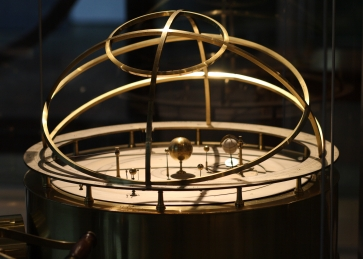
\includegraphics[scale=0.1]{./img/orrery-main.jpg}}
\end{center}

Though the Greeks had working planetaria, the first orrery that was a planetarium of the modern era was produced in 1704, and one was presented to the Earl of Orrery — whence came the name. They are typically driven by a clockwork mechanism with a globe representing the Sun at the centre, and with a planet at the end of each of the arms.


\pagebreak

\chapter*{The Idea}
\section*{Initial Design}
Our intial design that we made in \textbf{Inkscape} looked somewhat like this:
\begin{center}
\setlength\fboxsep{2pt}
\setlength\fboxrule{0pt}
\fbox{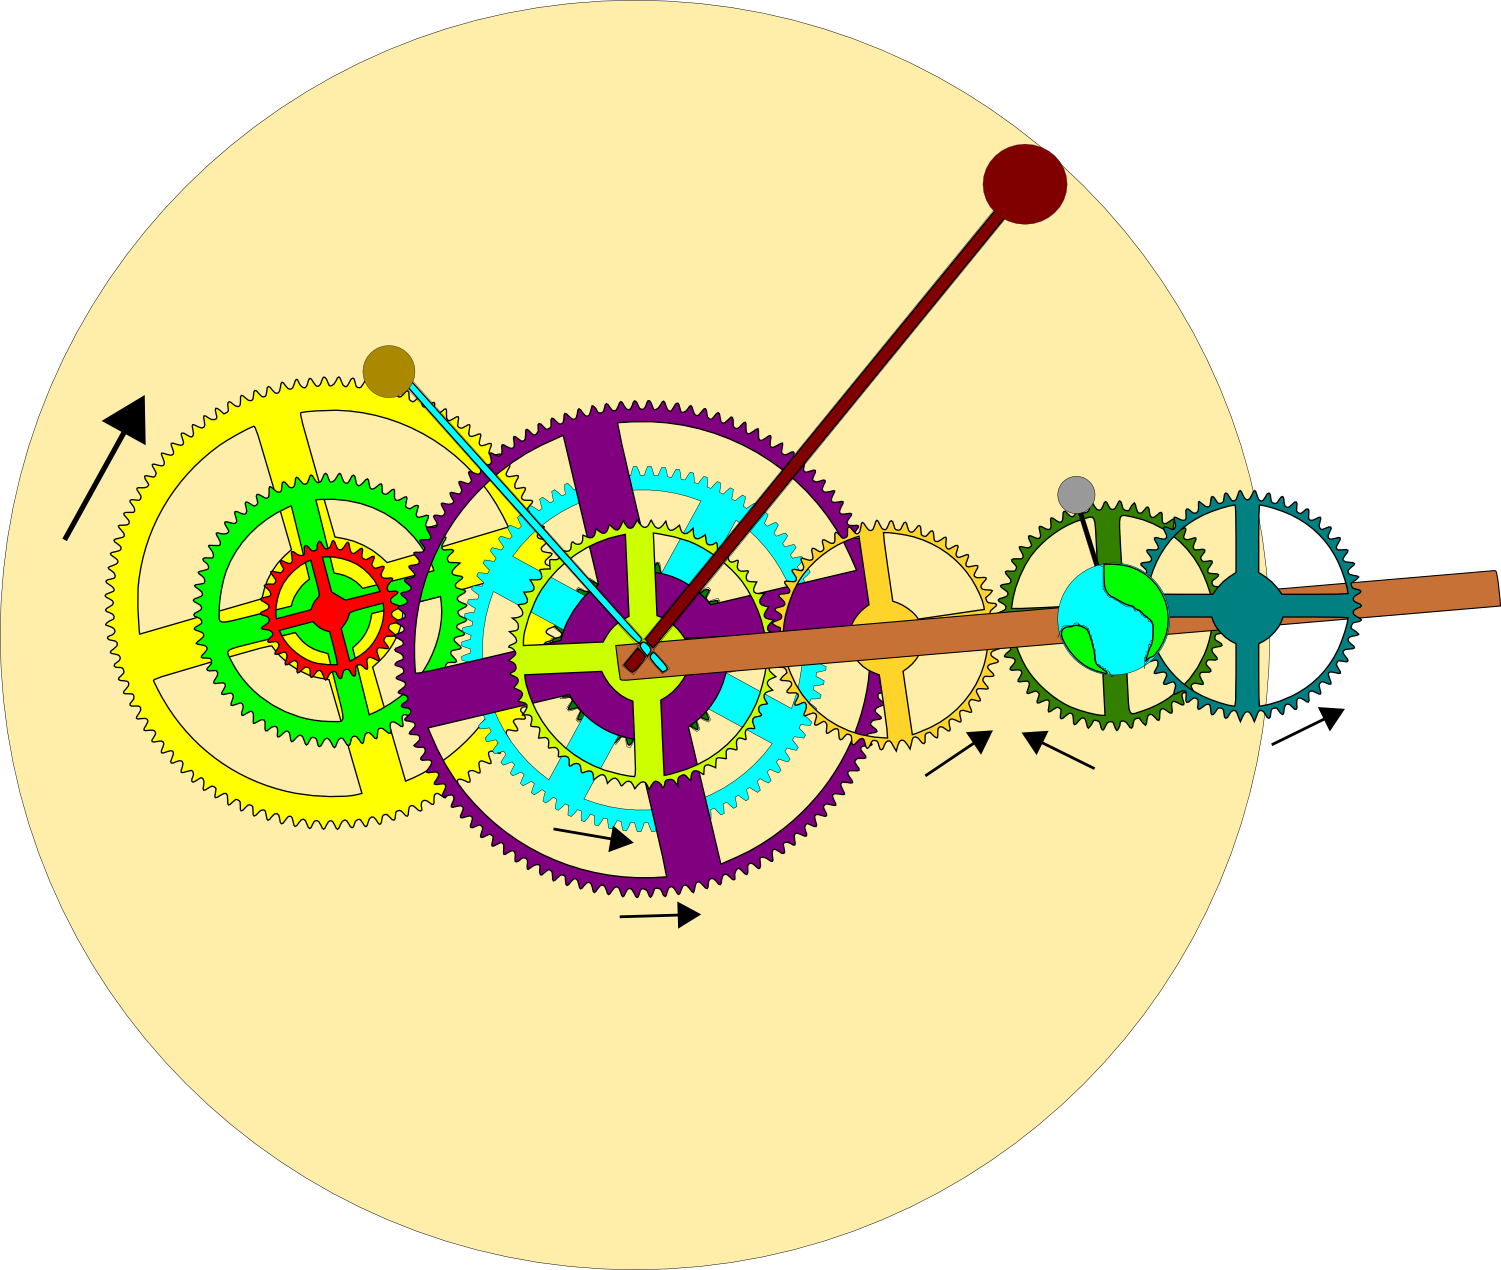
\includegraphics[scale=0.1]{./img/svg.png}}
\end{center}
Here, one of the gears in the center (say gear A) was driving one of the planets and another gear attached to it (say gear B). On top of gear B, another gear (gear C) was welded which in turn drove another gear with the same center as gear A. The angular velocity of this gear wasn't the same as A. This gear drove another planet. In this way, changing the angular velocities as a function of gear radii, we could simulate a part of the solar system. FOr the moon, we carried forward the gear motion from the center through a series of gears and attached a rod with a sphere, with a gear with the same center as the earth.

The system simulated through this arrangement assumed perfectly circular orbits, i.e. we neglected that the actual celestial orbits are a bit elliptical. Also, since the scope for error in calculations in Box2D is quite high, the system simulated by us doesn't take the exact ratios of orbits. Relatively, we tried to simulate the solar system as it is. For example the Earth revolves slower than Venus and Jupiter slower than the Earth. This has been incorporated in our design.

\section*{Deviation from the Original Design}
During the course of doing this project, we learnt a lot more than what we knew initially. Hence, we continuously modified our design to reach to the final output, that looks like this:
\begin{center}
\setlength\fboxsep{2pt}
\setlength\fboxrule{1pt}
\fbox{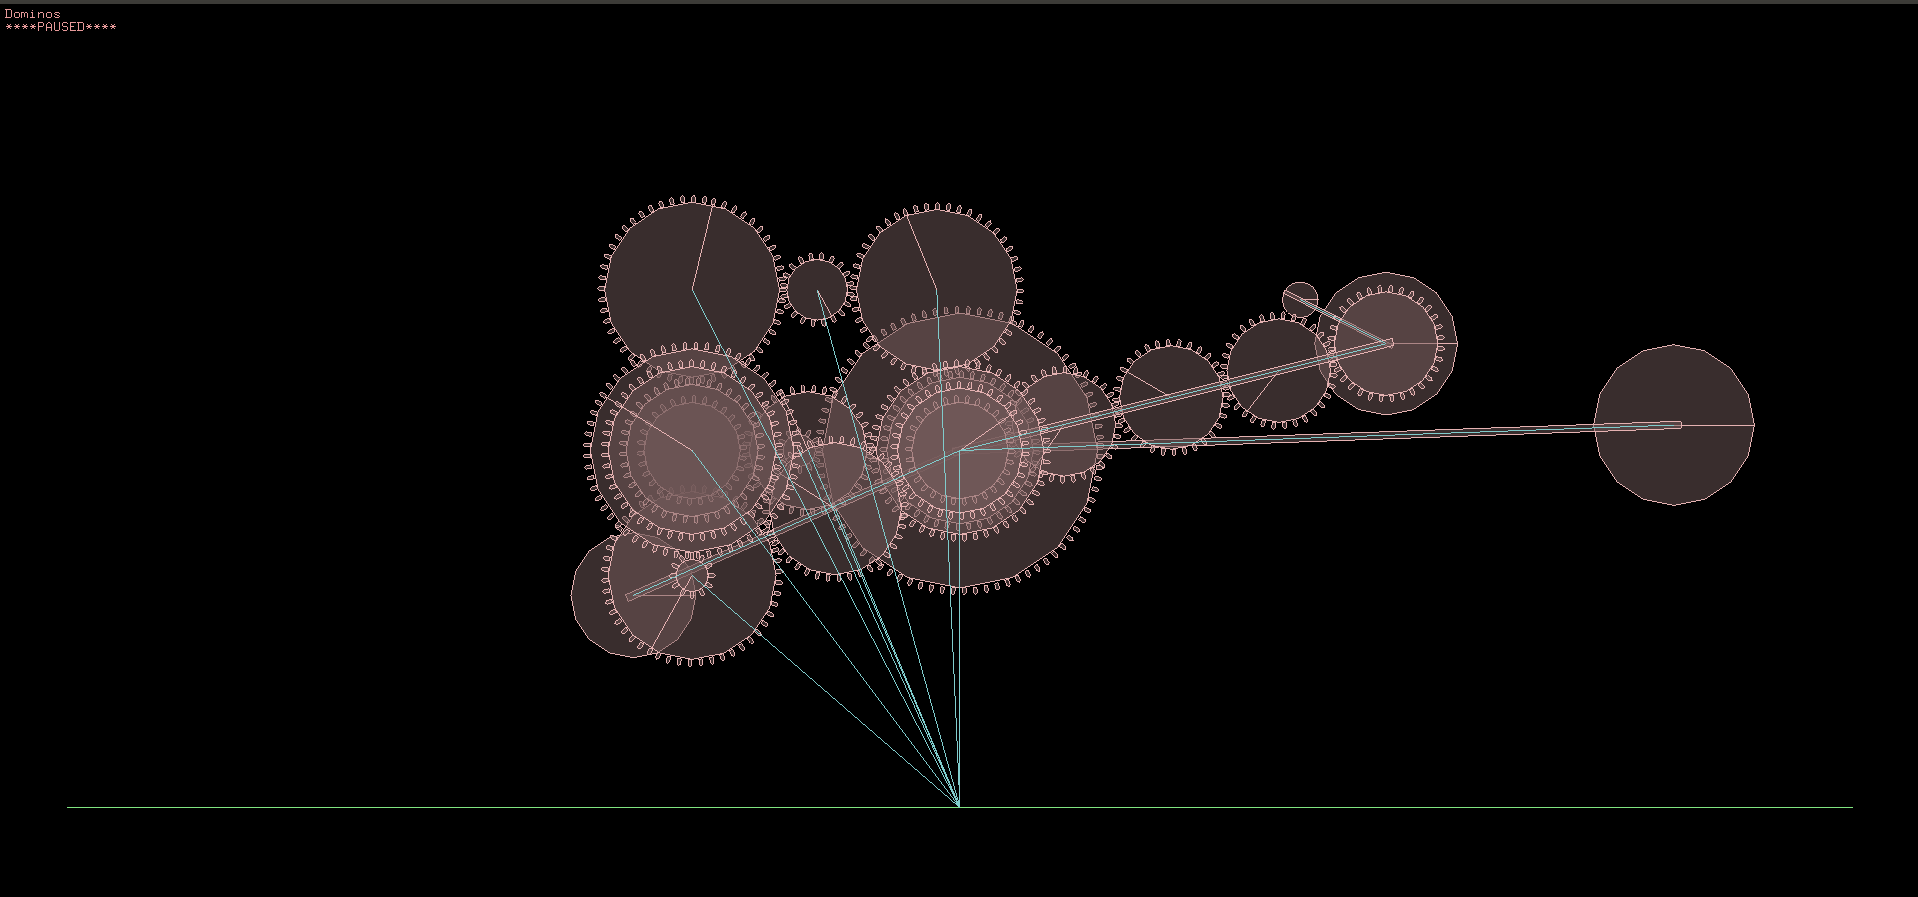
\includegraphics[scale=0.2]{./img/gui.png}}
\end{center}
Basically, the concept is the same. The only difference being, to prevent cluttering, we modified the conveyor-gear (the gears that transfer motion) positions. 
%I have to write modifications here.

\pagebreak
\chapter*{Points of Interest}
Simulating a natural phenomenon via a mechanical simulation is in fact pretty intersting. Whereas the actual solar system works on gravitational pull between celestial bodies, this system is purely contact driven. 

\bibliography{report}

\end{document}
}
